\documentclass[a4paper, 12pt]{article}
\usepackage[utf8]{inputenc}
\usepackage[english,swedish]{babel}
%\usepackage{cite}
\usepackage{hyperref}
\usepackage[
    backend=biber,
   % style=authoryear-icomp,
    sortlocale=se_sv,
    natbib=true,
    url=true,
    doi=true,
    eprint=true
]{biblatex}
%\usepackage[backend=bibtex]{biblatex}
\addbibresource{main.bib}
%\usepackage{times}

\usepackage{tikz}
\usetikzlibrary{shadows}
\newcommand*\key[1]{%
  \tikz[baseline=(key.base)]
    \node[%
      draw,
      fill=white,
      drop shadow={shadow xshift=0.25ex,shadow yshift=-0.25ex,fill=black,opacity=0.75},
      rectangle,
      rounded corners=2pt,
      inner sep=1pt,
      line width=0.5pt,
      font=\scriptsize\sffamily
    ](key) {#1\strut}
  ;
}

\title{Kassa\\\large en enkel kassa mjukvara}
\author{Sam Sadeghi SY17}
\date{2019/2020}

 
\begin{document}
\begin{titlepage}
\maketitle
\end{titlepage}

\selectlanguage{english}

\begin{abstract}

\end{abstract}
\selectlanguage{swedish}
\newpage
\tableofcontents
\newpage

\section{Inledning}
Ibland hjälper jag min farbror i hans livsmedel butik. 
Där får jag använd använda mig av kassaapparaten. 
Programmet som kassaapparaten på farbrors butik kör är långsamt och jag tänkte att jag skulle kunna göra ett liknande program som kör snabbare genom att endast ha med de nödvändigaste funktionerna.

\subsection{Syfte}

I skapandet av det här programmet ska jag lära mig hur man gör ett grafisk program med hjälp av programmerings språket Python och gränssnitsverktyget Tkinter. 

\subsection{Mål}

Vid slutet av arbetet ska jag ha ett enkelt kassa program som kan räkna ihop summan av flera varor samt hur mycket moms som skall betala beroende på varans typ. Programmet skall även kunna skriva ut ett kvitto 

\subsection{Metod}

Redskap jag kommer använda är


Vim:\\
Vim är ett text redigerings program som körs i konsolen.
Det finns massor med fördelar med Vim.
En av dessa fördelar är att den inte tar lika mycket resurser att köra Vim som till exempel Visual Studio men det i sig är inte så viktigt utan den största anledningen till varför jag jag använde Vim för att skriva det här programmet är att jag har vant mig vid Vims massor med tangentbords-genvägar och det hjälper mig skriva snabbare inte bara det utan jag är också väldigt bekväm med att konfigurera Vim så att lättare kan skriva.
Ett av dessa konfigurationer jag har gjort för att underlätta mitt skapande av programmet är att jag har gjort så att när jag trycker ner på \key{Ctrl } och \key{W} samtidigt så startar den programmet. Andra program kan säkert görande någonting liknade eller kanske till och med kommer inbyggt med en sådan funktion men i Vim får jag göra det det själv som får mig att bättre förstå vad som händer i bakgrunden och som sagt tidigare är jag mycket bekvämare med Vim än vad jag är med andra text redigerings program


Python:\\
% läs mer om TIOBE
% läs https://medium.com/@mindfiresolutions.usa/python-7-important-reasons-why-you-should-use-python-5801a98a0d0b
Python är ett programmeringsspråk.
Jag valde just Python för att skriva det här programmet för att jag ser det väldigt ofta i min omgivning.
Enligt TIOBE indexet \cite{TIOBE} är Python det tredje populäraste språket och dess popularitet värkar öka (se figur \ref{fig:index_python}) till skillnad från språket som ligger på första plats det vill säga Java (se figur \ref{fig:index_java}) och ju populärare ett programmeringsspråk är så finns det fler projekt som är skrivna i de programmeringsspråket därför tycker jag att det är värt att lära sig /skriva i  Python.


\begin{figure}[h!]
  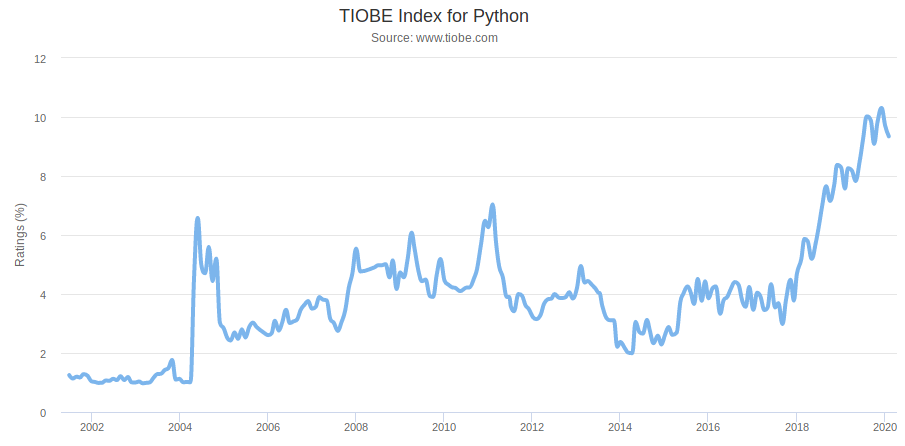
\includegraphics[width=\linewidth]{img/TIOBE_python.png}
  \caption{TIOBE index för python}
  \label{fig:index_python}
\end{figure}
\begin{figure}[h!]
  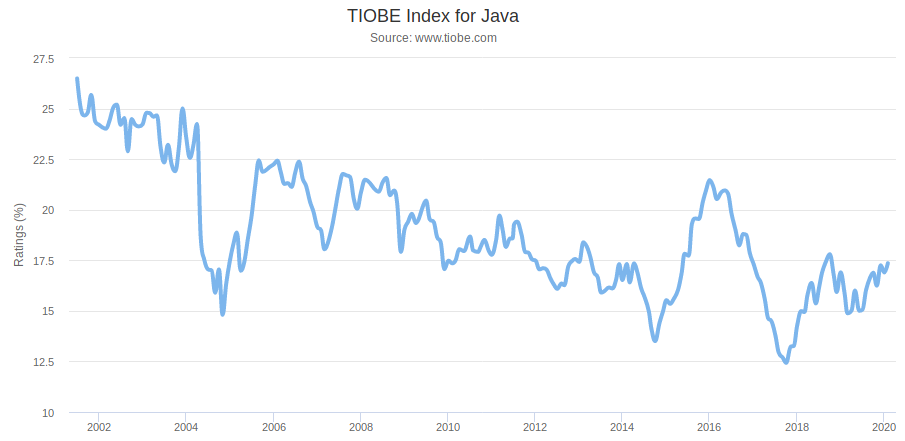
\includegraphics[width=\linewidth]{img/TIOBE_java.png}
  \caption{TIOBE index för java}
  \label{fig:index_java}
\end{figure}


Tkinter/TK:\\
Tkinter är en API för att använda TK i Python. 
TK är grafiskt gränssnits verktyg som fungerar på Windows, MacOS och Linux. 
Jag valde Tkinter på grund av att den fungerar på dom tre vanligare operativsystemen.
Tkinter kommer 


FPDF:\\
FPDF är ett programbibliotek för att generera PDF filer.
PDF filer är dokument filer som är optimerade för att skrivas ut.


Github och Git:\\
Github är en webbserver med fokus på program utveckling. 
Github använder sig av version kontroll programmet Git. 
Git gör det enkelt för mig att se vad jag har gjort och när jag har gjort det.
Git tillsammans med Github låter mig jobba på programmet var jag än är utan att vara uppkopplad till internet


Tutorialpoints sida på Python GUI Programming:\\
Tutorialpoints sida på Python GUI Programming är en webbsida som har i syfte att lära hur man använder TKinter.
Jag valde att använda Tutorialpoints sida istället för den officiella TKinter manualen efter som Tutorialpoints sida är mycket enklare att hitta information på. Det finns en lista på alla Widgets och en kort beskrivning av vad dem används för; du kan klicka på namnet av en widget du vill veta mer om och du tas till en sida där du får veta syntaxen och alla tillval för widgeten du klickat på.

\section{Utförande}

När jag börja projektet hade jag aldrig tidigare skrivit program i Python och det ända grafiska gränssnit jag tidigare använt var HTML på Webben så det första jag behövde göra var att lära mig.
Youtube videon ''How to Program a GUI Application (with Python Tkinter)!'' av Keith Galli\cite{yt:galli} användes för att få en förståelse av hur man gör grafiska program med Tkinter och python. 

Först behövdes ett sätt att skriva in siffror i programmet.
Man skulle kunna använda nummer knapparna på tangentbordet men eftersom ska kunna användas med endast en pekskärm så behövdes nummer knappar på skärmen, Detta gjorde jag genom att att skapa tio knappar (från 0 till 9)  och placera dom i en 3 gånger 3 rutnät med en stor knap för noll längst ner (se figur \ref{fig:numpad} ).


\begin{figure}[h!]
  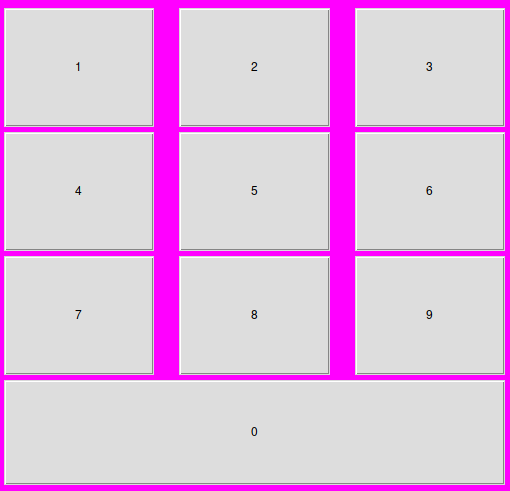
\includegraphics[width=\linewidth]{img/numpad.png}
  \caption{hur nummer knapparna ser ut}
  \label{fig:numpad}
\end{figure}

Därefter behövdes det ett sätt att se vad för nummer man skrivit; för det användes det en lable som döptes till text tillsammans med en global variabel som deklarerades med namnet num.
Num är noll när programmet startar men när en nummer knapp trycks så körs en funktion vid namnet knapp\_tryck med värdet på knappen; funktionen kommer sedan att multiplicera num med tio, addera värdet den fick in till num och tillslut visa det nya värdet för num på text. 
Nu kan användaren skriva in siffror i programmet men det saknas ett sätt att ta bort eller ångra siffror man skrivit därför implementerades till en knapp som raderar den sista siffran på talet och en knapp som tar bort hela talet.
Knappen som tar bort sista siffran är märkt med symbolen ''\textless'' och fungerar genom att kalla på funktionen knapp\_del. Funktionen knapp\_del fungerar på så sätt att den konverterar num till en sträng (detta görs för att det är lättare att kolla storleken och ta bort sista karaktären av en sträng). 
När num har konverterats till en sträng så kontrolleras det om num har fler än en karaktär i så fall tas den sista karaktären bort; om num bara har en karaktär kommer num sättas till noll.
Knappen som tar bort hela talet har bokstaven ''C'' på sig och kallar på funktionen knapp\_clear när den är tryckt. Knapp\_clear är en enkel funktion som byter värdet av num till noll.


\section{Resultat}

\section{Diskussion}

\section{Slutsats}

\newpage 

%\bibliography{main}{}
%\bibliographystyle{ieeetr}

\printbibliography

\end{document}
